% code generated by https://www.mathcha.io/editor#


% Gradient Info
  
\tikzset {_fl3j1z7ci/.code = {\pgfsetadditionalshadetransform{ \pgftransformshift{\pgfpoint{0 bp } { 0 bp }  }  \pgftransformscale{1 }  }}}
\pgfdeclareradialshading{_ajvec99hy}{\pgfpoint{0bp}{0bp}}{rgb(0bp)=(0,0,0);
rgb(0.17857142857142858bp)=(0,0,0);
rgb(25bp)=(1,1,1);
rgb(400bp)=(1,1,1)}
\tikzset{_c47t8m2b3/.code = {\pgfsetadditionalshadetransform{\pgftransformshift{\pgfpoint{0 bp } { 0 bp }  }  \pgftransformscale{1 } }}}
\pgfdeclareradialshading{_kz6fsyt8x} { \pgfpoint{0bp} {0bp}} {color(0bp)=(transparent!27);
color(0.17857142857142858bp)=(transparent!27);
color(25bp)=(transparent!0);
color(400bp)=(transparent!0)} 
\pgfdeclarefading{_sdra5fwgv}{\tikz \fill[shading=_kz6fsyt8x,_c47t8m2b3] (0,0) rectangle (50bp,50bp); } 
\tikzset{every picture/.style={line width=0.65pt}} %set default line width to 0.75pt        

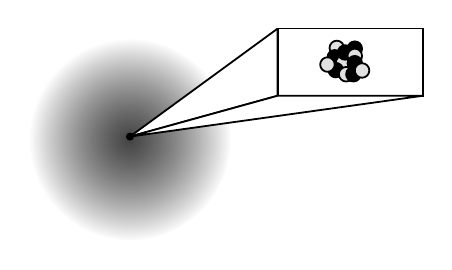
\begin{tikzpicture}[x=0.75pt,y=0.75pt,yscale=-1,xscale=1]
%uncomment if require: \path (0,300); %set diagram left start at 0, and has height of 300

%Shape: Circle [id:dp5031363586176847] 
\draw  [fill={rgb, 255:red, 0; green, 0; blue, 0 }  ,fill opacity=1 ] (353.67,159.68) .. controls (353.67,157.75) and (355.23,156.18) .. (357.17,156.18) .. controls (359.1,156.18) and (360.67,157.75) .. (360.67,159.68) .. controls (360.67,161.61) and (359.1,163.18) .. (357.17,163.18) .. controls (355.23,163.18) and (353.67,161.61) .. (353.67,159.68) -- cycle ;
%Shape: Circle [id:dp6021592429793765] 
\draw  [fill={rgb, 255:red, 225; green, 225; blue, 225 }  ,fill opacity=1 ] (345,159.33) .. controls (345,157.4) and (346.57,155.83) .. (348.5,155.83) .. controls (350.43,155.83) and (352,157.4) .. (352,159.33) .. controls (352,161.27) and (350.43,162.83) .. (348.5,162.83) .. controls (346.57,162.83) and (345,161.27) .. (345,159.33) -- cycle ;
%Shape: Circle [id:dp03262422408388033] 
\path  [shading=_ajvec99hy,_fl3j1z7ci,path fading= _sdra5fwgv ,fading transform={xshift=2}] (200,203.5) .. controls (200,176.53) and (221.86,154.67) .. (248.83,154.67) .. controls (275.8,154.67) and (297.67,176.53) .. (297.67,203.5) .. controls (297.67,230.47) and (275.8,252.33) .. (248.83,252.33) .. controls (221.86,252.33) and (200,230.47) .. (200,203.5) -- cycle ; % for fading 
 \draw  [color={rgb, 255:red, 255; green, 255; blue, 255 }  ,draw opacity=1 ] (200,203.5) .. controls (200,176.53) and (221.86,154.67) .. (248.83,154.67) .. controls (275.8,154.67) and (297.67,176.53) .. (297.67,203.5) .. controls (297.67,230.47) and (275.8,252.33) .. (248.83,252.33) .. controls (221.86,252.33) and (200,230.47) .. (200,203.5) -- cycle ; % for border 

%Shape: Circle [id:dp6125886336785793] 
\draw  [fill={rgb, 255:red, 0; green, 0; blue, 0 }  ,fill opacity=1 ] (247.37,202.04) .. controls (247.37,201.23) and (248.02,200.57) .. (248.83,200.57) .. controls (249.64,200.57) and (250.3,201.23) .. (250.3,202.04) .. controls (250.3,202.84) and (249.64,203.5) .. (248.83,203.5) .. controls (248.02,203.5) and (247.37,202.84) .. (247.37,202.04) -- cycle ;
%Shape: Rectangle [id:dp737374784788116] 
\draw   (320,150) -- (390,150) -- (390,182.36) -- (320,182.36) -- cycle ;
%Straight Lines [id:da9404773687410686] 
\draw [fill={rgb, 255:red, 255; green, 255; blue, 255 }  ,fill opacity=1 ]   (320,150) -- (320,182.36) -- (248.83,202.04) ;
%Shape: Polygon [id:ds005534302931645474] 
\draw  [fill={rgb, 255:red, 255; green, 255; blue, 255 }  ,fill opacity=1 ] (320,182.36) -- (390,182.36) -- (248.83,202.04) -- cycle ;
%Shape: Circle [id:dp39755043985132055] 
\draw  [fill={rgb, 255:red, 0; green, 0; blue, 0 }  ,fill opacity=1 ] (344,163.83) .. controls (344,161.9) and (345.57,160.33) .. (347.5,160.33) .. controls (349.43,160.33) and (351,161.9) .. (351,163.83) .. controls (351,165.77) and (349.43,167.33) .. (347.5,167.33) .. controls (345.57,167.33) and (344,165.77) .. (344,163.83) -- cycle ;
%Shape: Circle [id:dp4473204849748251] 
\draw  [fill={rgb, 255:red, 225; green, 225; blue, 225 }  ,fill opacity=1 ] (348,166.51) .. controls (348,164.58) and (349.57,163.01) .. (351.5,163.01) .. controls (353.43,163.01) and (355,164.58) .. (355,166.51) .. controls (355,168.45) and (353.43,170.01) .. (351.5,170.01) .. controls (349.57,170.01) and (348,168.45) .. (348,166.51) -- cycle ;
%Shape: Circle [id:dp4488461328919484] 
\draw  [fill={rgb, 255:red, 0; green, 0; blue, 0 }  ,fill opacity=1 ] (349,161.5) .. controls (349,159.57) and (350.57,158) .. (352.5,158) .. controls (354.43,158) and (356,159.57) .. (356,161.5) .. controls (356,163.43) and (354.43,165) .. (352.5,165) .. controls (350.57,165) and (349,163.43) .. (349,161.5) -- cycle ;
%Shape: Circle [id:dp7389549254976258] 
\draw  [fill={rgb, 255:red, 225; green, 225; blue, 225 }  ,fill opacity=1 ] (353.67,163.18) .. controls (353.67,161.25) and (355.23,159.68) .. (357.17,159.68) .. controls (359.1,159.68) and (360.67,161.25) .. (360.67,163.18) .. controls (360.67,165.11) and (359.1,166.68) .. (357.17,166.68) .. controls (355.23,166.68) and (353.67,165.11) .. (353.67,163.18) -- cycle ;
%Shape: Circle [id:dp479134066231107] 
\draw  [fill={rgb, 255:red, 0; green, 0; blue, 0 }  ,fill opacity=1 ] (344.5,170.01) .. controls (344.5,168.08) and (346.07,166.51) .. (348,166.51) .. controls (349.93,166.51) and (351.5,168.08) .. (351.5,170.01) .. controls (351.5,171.95) and (349.93,173.51) .. (348,173.51) .. controls (346.07,173.51) and (344.5,171.95) .. (344.5,170.01) -- cycle ;
%Shape: Circle [id:dp4479985418514103] 
\draw  [fill={rgb, 255:red, 225; green, 225; blue, 225 }  ,fill opacity=1 ] (340.5,167.33) .. controls (340.5,165.4) and (342.07,163.83) .. (344,163.83) .. controls (345.93,163.83) and (347.5,165.4) .. (347.5,167.33) .. controls (347.5,169.27) and (345.93,170.83) .. (344,170.83) .. controls (342.07,170.83) and (340.5,169.27) .. (340.5,167.33) -- cycle ;
%Shape: Circle [id:dp7971297276833167] 
\draw  [fill={rgb, 255:red, 0; green, 0; blue, 0 }  ,fill opacity=1 ] (353.67,166.68) .. controls (353.67,164.75) and (355.23,163.18) .. (357.17,163.18) .. controls (359.1,163.18) and (360.67,164.75) .. (360.67,166.68) .. controls (360.67,168.61) and (359.1,170.18) .. (357.17,170.18) .. controls (355.23,170.18) and (353.67,168.61) .. (353.67,166.68) -- cycle ;
%Shape: Circle [id:dp5729729111609032] 
\draw  [fill={rgb, 255:red, 225; green, 225; blue, 225 }  ,fill opacity=1 ] (349.5,172) .. controls (349.5,170.07) and (351.07,168.5) .. (353,168.5) .. controls (354.93,168.5) and (356.5,170.07) .. (356.5,172) .. controls (356.5,173.93) and (354.93,175.5) .. (353,175.5) .. controls (351.07,175.5) and (349.5,173.93) .. (349.5,172) -- cycle ;
%Shape: Circle [id:dp07629231382977153] 
\draw  [fill={rgb, 255:red, 0; green, 0; blue, 0 }  ,fill opacity=1 ] (353,172) .. controls (353,170.07) and (354.57,168.5) .. (356.5,168.5) .. controls (358.43,168.5) and (360,170.07) .. (360,172) .. controls (360,173.93) and (358.43,175.5) .. (356.5,175.5) .. controls (354.57,175.5) and (353,173.93) .. (353,172) -- cycle ;
%Shape: Circle [id:dp14599951094051478] 
\draw  [fill={rgb, 255:red, 225; green, 225; blue, 225 }  ,fill opacity=1 ] (357.17,170.18) .. controls (357.17,168.25) and (358.73,166.68) .. (360.67,166.68) .. controls (362.6,166.68) and (364.17,168.25) .. (364.17,170.18) .. controls (364.17,172.11) and (362.6,173.68) .. (360.67,173.68) .. controls (358.73,173.68) and (357.17,172.11) .. (357.17,170.18) -- cycle ;
%Straight Lines [id:da98323072818843] 
\draw    (248.83,202.04) -- (320,150) ;




\end{tikzpicture}
